\section{Methodologies and Implementation}
Starting from the Yellow-Spaceship game \cite{Yellow-Spaceship}, we have adapted the code to our needs.
In particular, we have modified the code that reads the action from the user keyboard in order to be
able to substitute the user input with an action computed by a program and apply it to the game.
The controlling action can be computed by an ANN trained using NEAT, or by a tree-based program evolved 
using GP, passing them the appropriate information about the current state of the game.
Moreover, the possibility to not show the game has been introduced in order to speed up the execution.

The inputs from the game environment for both NEAT and GP individuals are the following:
the $x$ coordinate of the battleship; the velocity of the battleship;
the $x$ coordinate of the first and second alien (if any, otherwise they are set to 0);
the $x$ and $y$ coordinates of the first and second closest lasers (if any, otherwise they are set to 0);
the $x$ coordinate of the enemy spaceship (if any, otherwise it is set to 0).
In this way, there are a total of 9 arguments of type float passed to the individuals as input that
can be used to decide the action to perform. 
The performance of an individual can be evaluated based on how much it moves on in the game.

The fitness function for the individuals of both the algorithms that we decided to use can be
formulated as follows:
\begin{equation}
\begin{split}
    fitness = & alien\_kills * 10 + \\
              & enemy\_spaceship\_kills * 50 + \\
              & \sum_{h \in battleships\_healths}^{} \frac{h}{50} + \\
              & \sum_{a \in aliens}^{} \frac{cur\_alien\_health - a.health}{cur\_alien\_health} * 10 + \\
              & \sum_{s \in enemy\_spaceships}^{} 50 - s.health
\end{split}
\end{equation}
where $alien\_kills$ is the number of aliens killed, 
$enemy\_spaceship\_kills$ is the number of enemy spaceships killed,
$battleship\_healths$ is a vector of battleship health at the beginning of each level and
$cur\_alien\_health$ is the initial alien health at the last level reached. 

The fitness function should be maximized and takes into account the number of aliens and
enemy spaceships killed, the battleship health at each level and the health of aliens and
enemy spaceships at the last level reached. There is no intermediate reward and the overall
fitness is returned at the end of simulation.

In order to handle cases in which the simulation takes too much time because the battleship
is not killed, we introduced a maximum threshold on the number of frames: the game will be
stopped after $1$ million frames. The threshold permits to prevent the execution from getting
stuck and also incentivizes the NEAT and GP algorithms to learn how to reach higher levels
with the same number of frames. When the best individual execution is shown,
this limit is released in order to obtain the actual fitness without interrupting the game.

To speed up the evolution process, individuals are evaluated only every 10 frames to obtain
the action to perform: the previous action is applied for the rest of 9 frames. This value
should be sufficient to permit the individual to have enough control over the battleship
actions and not be killed by enemies. In this way the evaluation process proceeds about 10
times faster and the battleship movements look smoother.


\subsection{NEAT}
The implementation is based on the NEAT-Python library \cite{NEAT-Python}, which is a pure Python
implementation of NEAT, with no dependencies other than the Python standard library.
We decided to evolve a feed forward neural network with the possibility of learning skip
connections instead of a recurrent neural network since the actual state of the game is
sufficient to train the neural network and no more information is required. The network has 6
output nodes and each of them encodes a particular action that the agent has to perform:
go left; go left and fire; stay still; stay still and fire; go right; go right and fire.
The output node with the maximum value is taken to decide the action to perform.

We decided to adopt the following algorithm parameters:
\begin{itemize}
    \item $num\_runs = 10$, $num\_generations = 200$ and $no\_fitness\_termination = True$
    \item $pop\_size = 100$ and $reset\_on\_extinction = True$
    \item $activation = sigmoid$ and $aggregation = sum$
    \item $conn\_add\_prob = 0.5$ and $conn\_delete\_prob = 0.5$
    \item $enabled\_default = True$ and $enabled\_mutate\_rate = 0.01$
    \item $feed\_forward = True$ and $initial\_connection = full\_nodirect$
    \item $node\_add\_prob = 0.2$ and $node\_delete\_prob = 0.2$
    \item $num\_inputs = 9$, $num\_hidden = 9$ and $num\_outputs = 6$
    \item $species\_fitness\_func = max$, $max\_stagnation = 20$ and $species\_elitism = 2$
    \item $elitism = 2$, $survival\_threshold = 0.2$ and $min\_species\_size = 2$
\end{itemize}

All the configuration parameters used by the algorithm can be modified in the configuration
file named 'configNEAT.txt' present in the root directory of the project.


\begin{figure*}[htbp]
\centerline{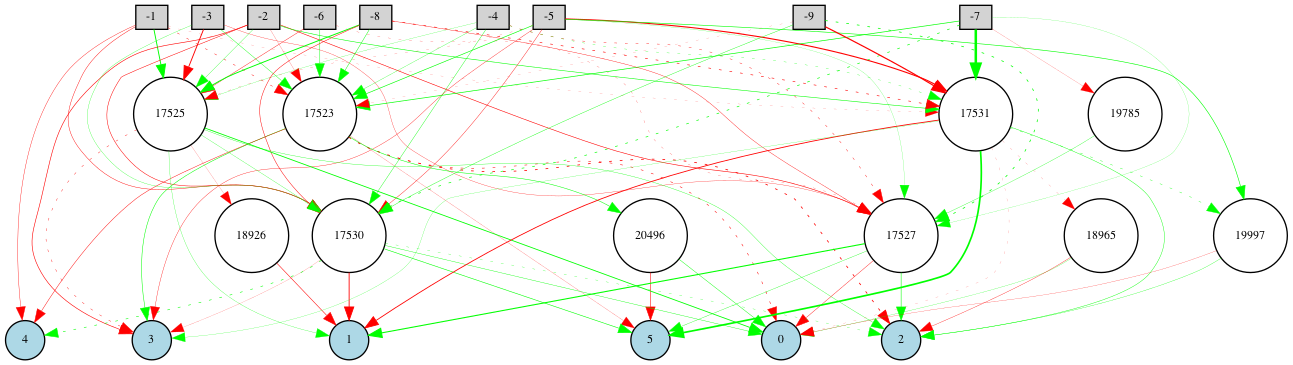
\includegraphics[scale=0.35]{NEAT_best.png}}
\caption{Best ANN generated by NEAT.}
\label{fig:NEAT_best}
\end{figure*}


\subsection{GP}
The implementation is based on the DEAP library \cite{DEAP}, which is a Python evolutionary
computation framework which provides the main blocks for building Genetic Programming
algorithms. Strongly typed genetic programming (STGP) is an enhanced version of genetic
programming which enforces data type constraints.

A tree-based program has been evolved using STGP. The output of the program is one of
the 6 encoded actions that the agent can perform. To encode the actions, we defined one
class for each of them with the following encoding:
A, go left; B, go left and fire; C, stay still; D, stay still and fire; E, go right; F, go right and fire.

The terminal set is composed of the action classes, some float values ($5$, $10$, $15$, $20$, $25$, $30$)
and the boolean values ("true", "false"). The function set is composed of the
boolean operators "greater than", "equal", "and", "or" and "negation", the arithmetic operators
"add", "subtract" and "multiply" and the "if-then-else" function that can outputs a float value or
an action class. Since the "if-then-else" function is the only function that outputs an action, it
should always be at the root of the tree.

We decided to adopt the following algorithm parameters:
\begin{itemize}
    \item $num\_runs = 10$ and $num\_generations = 200$
    \item $pop\_size = 100$
    \item $crossover\_prob = 0.5$
    \item $mutation\_prob = 0.5$
    \item $hof\_size = 4$
    \item $max\_tree\_size = 500$
    \item $max\_tree\_height = 10$
    \item As $expr\_init$ we used $gp.genFull$ with $min\_ = 1$ and $max\_ = 3$
    \item As $select$ we used $tools.selTournament$ with $tournsize = 7$
    \item As $mate$ we used $gp.cxOnePoint$
    \item As $expr\_mut$ we used $gp.genFull$ with $min\_ = 0$ and $max\_ = 2$
    \item As $mutate$ we used $gp.mutUniform$
    \item As $algorithm$ we used $deap.algorithms.eaSimple$
\end{itemize}

All the configuration parameters used by the algorithm can be modified in the configuration
file named 'configGP.txt' present in the root directory of the project.
